\documentclass[lang=en,mode=normal,device=normal,color=blue,12pt]{elegantnote}

\usepackage{amsmath,amssymb}
\usepackage{bbm}
\usepackage{tcolorbox}
\usepackage{graphicx}
\usepackage{booktabs}
\usepackage{subfig}
\usepackage{algorithm}
\usepackage{algpseudocode}
\usepackage[toc,page,title]{appendix}
\usepackage{hyperref}

\setlength{\parindent}{0pt}


\DeclareMathOperator*{\1}{\mathbbm{1}}
\DeclareMathOperator*{\E}{\mathbb{E}}
\DeclareMathOperator*{\D}{\mathcal{D}}
\DeclareMathOperator*{\R}{\mathbbm{R}}
\DeclareMathOperator*{\argmax}{arg\,max}
\DeclareMathOperator*{\argmin}{arg\,min}

\title{Study Note: Soft Actor Critic}

\author{Yanqing Wu}
%\author{Yanqing Wu\\[0.5cm]{Advisor: Prof. Hengshuai Yao}}
\institute{Viwistar Robotics}

\begin{document}
\maketitle

\newpage

Since some parts are not addressed directly from the literature, the explanations in this note are the best of my understanding.


\section{Introduction}


Model-free deep reinforcement learning (RL) algorithms are proven to work on decision making and control tasks. However, these methods are hindered by two major challenges: very high sample complexity (requires at least millions of steps of data collection) and brittle convergence properties (extremely sensitive to hyperparameters).
One cause for the high sample complexity (or poor sample efficiency) is on-policy learning. On-policy learning methods, such as TRPO, PPO, or A3C, require collecting new samples for each gradient step and which is extremely expensive.
To improve sample efficiency, we need to reuse past experience (or `experience replay' in literature), which requires off-policy algorithms  \cite{mnih2013playing}. However, off-policy variants based on soft Q-learning require complex approximate inference procedures in continuous action spaces. 
% https://web.stanford.edu/class/psych209/Readings/MnihEtAlHassibis15NatureControlDeepRL.pdf


Soft Actor Critic \cite{haarnoja2018soft}, or SAC, was introduced to provide both sample efficiency and stability in continuous action spaces, and extendability to complex and high-dimensional tasks. SAC is an off-policy actor-critic deep RL algorithm based on the maximum entropy framework. In this framework, the actor aims to maximize expected reward as well as entropy. That is, to succeed at the task while acting as randomly as possible. Prior deep RL methods based on this framework have been formulated as Q-learning methods. SAC combines off-policy updates with a stable stochastic actor-critic formulation.


\section{SAC}
%\url{https://spinningup.openai.com/en/latest/algorithms/sac.html}
%
%\url{https://towardsdatascience.com/soft-actor-critic-demystified-b8427df61665}
%
%\url{https://spinningup.openai.com/en/latest/spinningup/rl_intro.html}

\subsection{Implementation}

Three key components in SAC:

\begin{itemize}
\item An actor-critic architecture with separate policy and value function networks;
\item An off-policy formulation that enables reuse of previously collected data for efficiency;
\item Entropy maximization to enable stability and exploration.
\end{itemize}

The policy is trained with the \textbf{objective} to maximize the expected return and the entropy at the same time:
\[
J(\theta) = \sum_{t=1}^T \E_{(s_t, a_t) \sim \rho_{\pi_\theta}} [r(s_t, a_t) + \alpha \mathbb{H} (\pi_\theta(\cdot | s_t))]
\]
where $\mathbb{H}(\cdot)$ is the entropy measure and $\alpha$ (temperature parameter) controls how important the entropy term is.
The entropy maximization leads to policies that can (1) explore more and (2) capture multiple modes of near-optimal strategies (i.e., if there exist multiple options that seem to be equally good, the policy should assign each with an equal probability to be chosen).

Precisely, SAC aims to learn three functions:

\begin{itemize}
\item $\pi_\theta$, the policy with parameter $\theta$
\item $Q_w$, soft Q-value function parameterized by $w$
\item $V_\psi$, soft state-value function parameterized by $\psi$
\end{itemize}

\textbf{Soft Q-value} (or soft action value) and \textbf{soft state value} are defined as:
\begin{align*}
Q(s_t, a_t) &= r(s_t, a_t) + \gamma \mathbb{E}_{s_{t+1} \sim \rho_{\pi}(s)} [V(s_{t+1})] & \text{; according to Bellman equation.}\\
\text{where }V(s_t) &= \mathbb{E}_{a_t \sim \pi} [Q(s_t, a_t) - \underbrace{\alpha \log \pi(a_t | s_t)}_\text{entropy}] & \text{; soft state value function.}
\end{align*}
\[
\text{Thus, } Q(s_t, a_t) = r(s_t, a_t) + \gamma \mathbb{E}_{(s_{t+1}, a_{t+1}) \sim \rho_{\pi}} [Q(s_{t+1}, a_{t+1}) - \alpha \log \pi(a_{t+1} \vert s_{t+1})]
\]
$\rho_\pi (s_t)$ and $\rho_\pi(s_t, a_t)$ denote the state and state-action marginals of the trajectory (state) distribution included by a policy $\pi (a_t |s_t)$.

The \textbf{soft state value function} is trained to minimize the mean square error:
\begin{align*}
J_V(\psi) &= \mathbb{E}_{s_t \sim \mathcal{D}} [\frac{1}{2} \big( \underbrace{V_\psi(s_t)}_\text{value} - \mathbb{E}[\underbrace{Q_w(s_t, a_t)}_\text{target} - \underbrace{\log \pi_\theta(a_t \vert s_t)}_\text{entropy}] \big)^2] \\
\text{with gradient: }\nabla_\psi J_V(\psi) &= \nabla_\psi V_\psi(s_t)\big( V_\psi(s_t) - Q_w(s_t, a_t) + \log \pi_\theta (a_t \vert s_t) \big)
\end{align*}
where $\mathcal{D}$ is the replay buffer.

The \textbf{soft Q function} is trained to minimize the soft Bellman residual:
\begin{align*}
J_Q(w) &= \mathbb{E}_{(s_t, a_t) \sim \mathcal{D}} [\frac{1}{2}\big( Q_w(s_t, a_t) - \underbrace{(r(s_t, a_t) + \gamma \mathbb{E}_{s_{t+1} \sim \rho_\pi(s)}[V_{\bar{\psi}}(s_{t+1})])}_\text{target} \big)^2] \\
\text{with gradient: } \nabla_w J_Q(w) &= \nabla_w Q_w(s_t, a_t) \big( Q_w(s_t, a_t) - r(s_t, a_t) - \gamma V_{\bar{\psi}}(s_{t+1})\big)
\end{align*}
where $\bar{\psi}$ is the target value function which is the exponential moving average (or only gets updated periodically in a `hard' way), just like how the parameter of the target Q network is treated in DQN to stabilize the training.

SAC updates the policy to minimize the KL-divergence:
\begin{align*}
\pi_\text{new} 
&= \arg\min_{\pi' \in \Pi} D_\text{KL} \Big( \pi'(\cdot | s_t) \| \frac{\exp(Q^{\pi_\text{old}}(s_t, \cdot))}{Z^{\pi_\text{old}}(s_t)} \Big) \\[6pt]
&= \arg\min_{\pi' \in \Pi} D_\text{KL} \big( \pi'(\cdot | s_t) \| \exp(Q^{\pi_\text{old}}(s_t, \cdot) - \log Z^{\pi_\text{old}}(s_t)) \big) \\[6pt]
\text{objective for update: } J_\pi(\theta) &= \nabla_\theta D_\text{KL} \big( \pi_\theta(\cdot | s_t) \| \exp(Q_w(s_t, \cdot) - \log Z_w(s_t)) \big) \\[6pt]
&= \mathbb{E}_{a_t\sim\pi} \Big[ - \log \big( \frac{\exp(Q_w(s_t, a_t) - \log Z_w(s_t))}{\pi_\theta(a_t | s_t)} \big) \Big] \\[6pt]
&= \mathbb{E}_{a_t\sim\pi} [ \log \pi_\theta(a_t | s_t) - Q_w(s_t, a_t) + \log Z_w(s_t) ]
\end{align*}
where $\Pi$ is the set of potential policies that we can model our policy as to keep them tractable; e.g., $\Pi$ can be the family of Gaussian mixture distributions, expensive to model but highly expressive and still tractable.
$Z^{\pi_{\text{old}}}(s_t)$ is the partition function to normalize the distribution.
It is usually intractable but does not contribute to the gradient. How to minimize $J_\pi (\theta)$ depends our choice of $\Pi$.

This update guarantees that $Q^{\pi_\text{new}}(s_t, a_t) \geq Q^{\pi_\text{old}}(s_t, a_t)$, please check the proof on this lemma in the Appendix B.2 in \cite{haarnoja2018soft}.

Once we have defined the objective functions and gradients for soft action-state value, soft state value and the policy network, the soft actor-critic algorithm is as follows:
\begin{figure}[!ht]
  \centering
  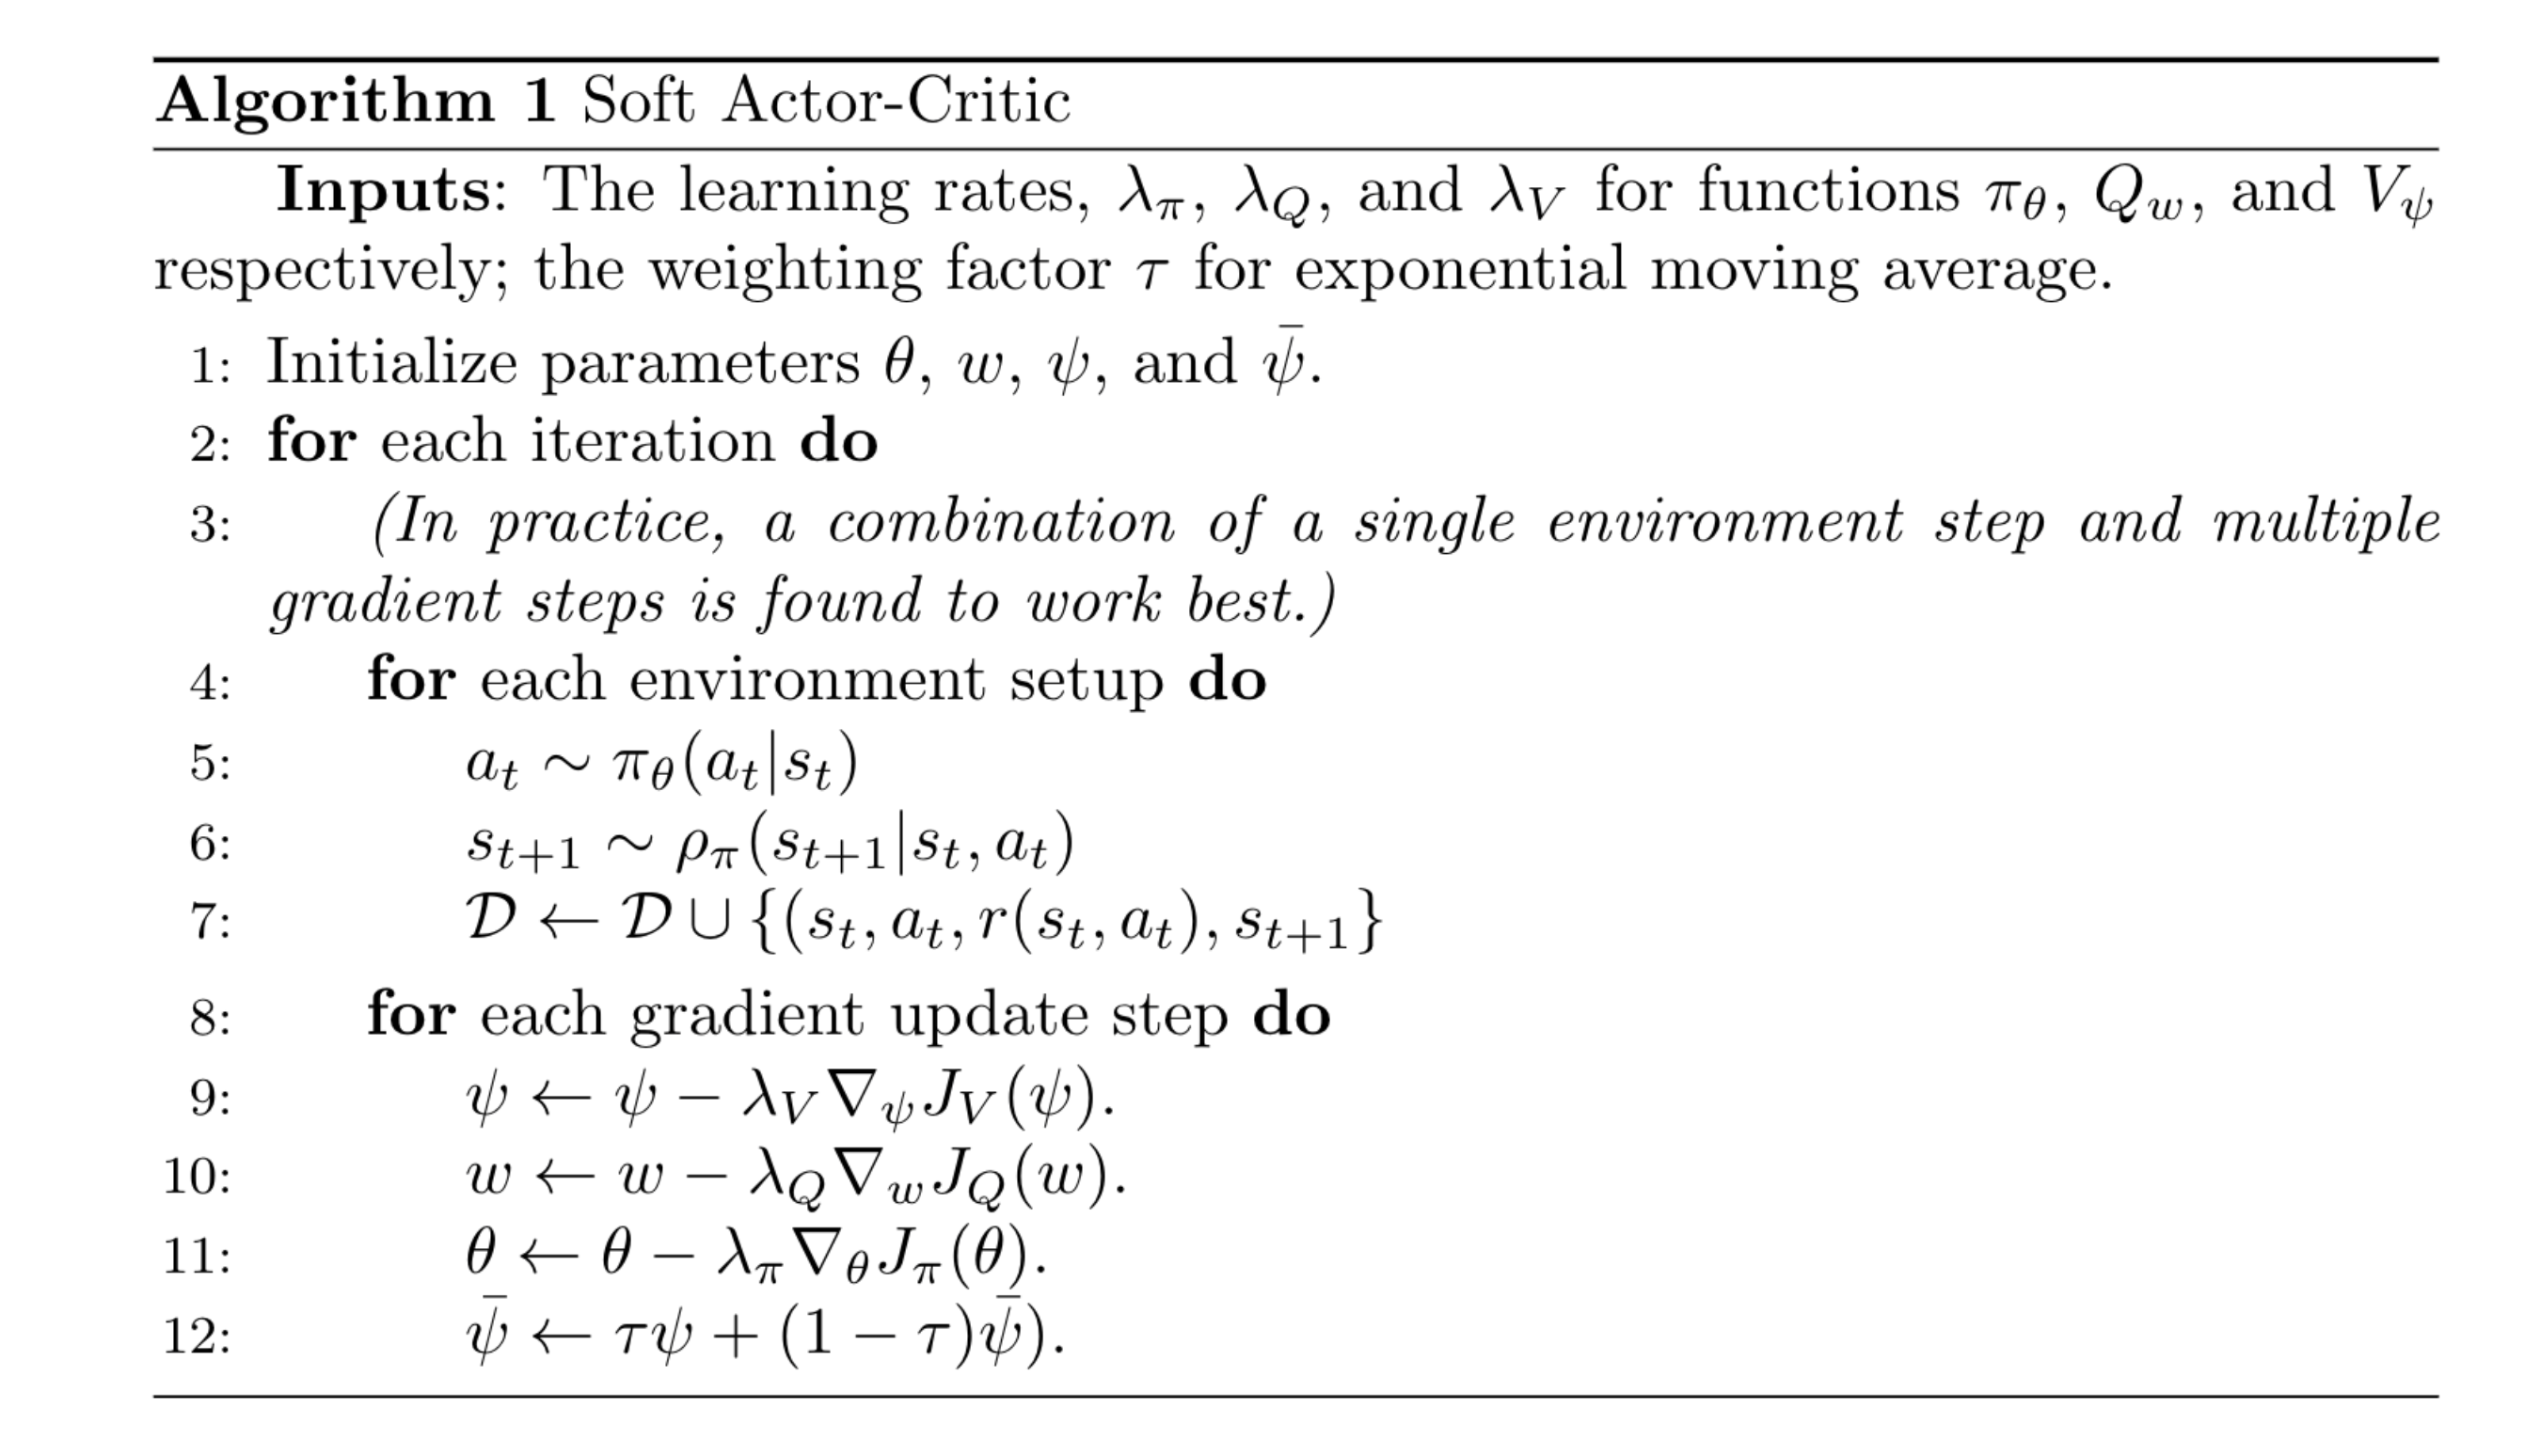
\includegraphics[width=0.9\linewidth]{SAC_algo.png}
  \caption{Screenshot of SAC algorithm}
  \label{fig:SAC_algo}
\end{figure}

\paragraph{Source Code}
\url{https://github.com/haarnoja/sac}

\subsection{SAC Improvement}

\subsubsection{SAC with automatically adjusted temperature}

SAC is brittle with respect to the temperature parameter.
Unfortunately it is difficult to adjust temperature, because the entropy can vary unpredictably both across tasks and during training as the policy becomes better.
An improvement on SAC formulates a constrained optimization problem: while maximizing the expected return, the policy should satisfy a minimum entropy constraint \cite{haarnoja2019soft}.


\section{Further reading}
%%%%%%%%%%%%%%%%%%%%%%%%%%
%%compute efficiency vs. sample efficiency, where SAC outperforms PPO in sample efficiency
%
\begin{itemize}
\item \href{https://www.youtube.com/watch?v=pg-lKy7JIRk}{L5 DDPG and SAC (Foundations of Deep RL Series) (by Pieter Abbeel)}
\begin{itemize}
\item ``you can think of SAC as maximum entropy version of DDPG'' by Pieter Abbeel
\end{itemize}
\item \href{https://www.youtube.com/watch?v=QASqaj_HUZw}{Lecture 19 Off-Policy, Model-Free RL: DQN, SoftQ, DDPG, SAC -- CS287-FA19 Advanced Robotics (by Pieter Abbeel)}
\item \href{https://www.youtube.com/watch?v=Y2XBiUtZo1k}{Lecture 20 Model-Based Reinforcement Learning -- CS287-FA19 Advanced Robotics at UC Berkeley (by Pieter Abbeel)}
\item DDPG: \url{https://arxiv.org/pdf/1509.02971.pdf}
\begin{itemize}
\item \url{https://spinningup.openai.com/en/latest/algorithms/ddpg.html}
\item \href{https://towardsdatascience.com/deep-deterministic-policy-gradient-ddpg-theory-and-implementation-747a3010e82f}{DDPG explained blog 1}, \href{https://lilianweng.github.io/lil-log/2018/04/08/policy-gradient-algorithms.html#ddpg}{DDPG explained blog 2}
\end{itemize}
\end{itemize}


%\section{Questions}
%
%\url{https://www.reddit.com/r/reinforcementlearning/comments/d8s33q/discounted_state_distribution/}



%%%%%%%%%%%%%%%%%%%%%%%%%%%%%%%%%%%%%%%%%%%%%%%
% Appendices
%%%%%%%%%%%%%%%%%%%%%%%%%%%%%%%%%%%%%%%%%%%%%%%

\newpage
\begin{appendices}

\section{Taxonomy of reinforcement learning algorithms}

\subsection{Model-free vs. Model-based}
\label{appendix:model-dep}

You may have seen `model' referring to neural networks like in supervised learning.
In RL, the term `model' in `model-free' or `model-based' does NOT refer to neural networks or other statistical learning models.
To avoid ambiguity, neural networks are referred as `function approximators' in RL, which are often employed to learn and generalize value functions (such as Q values that predicts total return given a state-action pair).

Model-based RL has an agent try to understand the environment and create a `model' represent it.
\textbf{The transition function (probability distribution) from states $T$ and the reward function $R$ are called the `model' of the environment} (or Markov decision process, MDP).
From this model, the agent has a reference and can \textit{plan} accordingly. Model-free agent does not learn a model but instead learn a policy directly.

A RL agent is not `model-based' even there is a model of the environment implemented. A RL agent have to explicitly reference the `model' to be `model-based':

\begin{itemize}
\item `model-free' algorithms: algorithms that purely sample from experience (e.g. Monte Carlo control, SARSA, Q-learning, Actor-Critic)
\begin{itemize}
\item They rely on real samples from the environment and never use generated predictions of next state and next reward to alter behaviour. They might sample from experience memory (e.g. replay buffer), which is close to being a model.
\end{itemize}
\item archetypical `model-based' algorithms: Dynamic Programming (e.g. Policy Iteration, Value Iteration)
\begin{itemize}
\item They use the model's predictions or distributions of enxt state and reward to calculate optimal actions. In DP specifically, the model must provide state transition probabilities, and expected reward from any state, action pair.
\end{itemize}
\item other `model-based' algorithms: basic TD learning that only uses state values
\begin{itemize}
\item To pick the optimal action, it needs to ask a model that predicts what will happen on each action and implement a policy like $\pi(s) = argmax_a \sum_{s',r} p(s',r|s,a)(r+v(s'))$ where probability function $p(s',r|s,a)$ is essentially the model.
\end{itemize}
\end{itemize}

In short, model-based RL algorithms use models and planning to solve RL problems; model-free methods are explicitly trial-and-error learners (almost the opposite of planning).

A simple check to see if an RL algorithm is model-based or model-free is: \textit{if, after learning, the agent can make predictions about what the next state and reward will be before it takes each action, it is a model-based RL algorithm. If it cannot, then it is a model-free algorithm}.

% roll-out: The standard use of “rollout” (also called a “playout”) is in regard to an execution of a policy from the current state when there is some uncertainty about the next state or outcome - it is one simulation from your current state. 


\subsection{On-policy vs. Off-policy}
\label{appendix:on-off-policy}

By Prof. Yao, the key difference between the two is whether we use generated action to interact with the environment.

\begin{itemize}
\item On-policy learning: the same policy that is evaluated and improved is \textit{also} used to select actions.
\item Off-policy learning: the policy that is evaluated and improved (called estimation policy) is different from the policy that is used to select actions (called behaviour policy).
\end{itemize}

The on-policy methods, like SARSA, expects that the actions in every state are chosen based on the current policy of the agent, that usually tends to exploit rewards. By doing so, the policy gets better when we update our policy based on the last rewards. But, if we update our policy based on stored transitions, like in experience replay, we are actually evaluating actions from a policy that is no longer the current one.

An advantage of this separation is that the estimation policy may be deterministic (e.g. greedy), while the behaviour policy can continue to sample all possible actions.
Hence, off-policy gives us better exploration and helps us use data samples more efficiently.

Within off-policy methods, there are two types: Q learning and Q-based policy gradient (or Q-based actor critic) \cite{ytbcs287}.

\subsection{Policy-based vs. Value-based}

\begin{itemize}
\item policy-based: we explicitly build a representation of a policy (mapping $\pi:s\rightarrow a$) and keep it in memory during learning
\item value-based: we don't store any explicit policy, only a value function. The policy is here implicit and can be derived directly from the value function (pick the action with the best value)
\item actor-critic: a mix of policy-based (actor) and value-based (critic).
\end{itemize}

\subsubsection{Q-learning vs. Policy Gradient}

A more specific and symbolic example of policy-based vs value-based methods is: Q-learning (value-balsed) and Policy Gradient (policy-based).

In a post by \cite{qlearningvspg}: Both methods are theoretically driven by the Markov Decision Process construct, and as a result use similar notation and concepts. In addition, in simple solvable environments you should expect both methods to result in the same - or at least equivalent - optimal policies.

However, they are actually different internally. The most fundamental differences between the approaches is in how they approach action selection, both whilst learning, and as the output (the learned policy). In Q-learning, the goal is to learn a single deterministic action from a discrete set of actions by finding the maximum value. With policy gradients, and other direct policy searches, the goal is to learn a map from state to action, which can be stochastic, and works in continuous action spaces.

As a result, policy gradient methods can solve problems that value-based methods cannot:
\begin{itemize}
\item Large and continuous action space. However, with value-based methods, this can still be approximated with discretisation - and this is not a bad choice, since the mapping function in policy gradient has to be some kind of approximator in practice.
\item Stochastic policies. A value-based method cannot solve an environment where the optimal policy is stochastic requiring specific probabilities, such as Scissor/Paper/Stone. That is because there are no trainable parameters in Q-learning that control probabilities of action, the problem formulation in TD learning assumes that a deterministic agent can be optimal.
\end{itemize}
However, value-based methods like Q-learning have some advantages too:
\begin{itemize}
\item Simplicity. You can implement Q functions as simple discrete tables, and this gives some guarantees of convergence. There are no tabular versions of policy gradient, because you need a mapping function $p(a|s,\theta)$ which also must have a smooth gradient with respect to $\theta$.
\item Speed. TD learning methods that bootstrap are often much faster to learn a policy than methods which must purely sample from the environment in order to evaluate progress.
\end{itemize}
There are other reasons why you might care to use one or other approach:
\begin{itemize}
\item You may want to know the predicted return whilst the process is running, to help other planning processes associated with the agent.
\item The state representation of the problem lends itself more easily to either a value function or a policy function. A value function may turn out to have very simple relationship to the state and the policy function very complex and hard to learn, or vice-versa.
\end{itemize}

Some state-of-the-art RL solvers actually use both approaches together, such as Actor-Critic. This combines strengths of value and policy gradient methods.



\section{Soft policy vs. Stochastic policy}

\begin{itemize}
\item deterministic policy, $\pi(s) = a$
\item stochastic policy, $\pi(a|s) = \mathbb{P}_\pi [A=a | S=s]$
\item soft policy, $\pi(a|s) = \mathbb{P}_\pi [A=a | S=s] > 0$
\end{itemize}

The term `soft policy' and `stochastic policy' are not interchangeable. Soft policy are always stochastic, but not all stochastic policies are soft policies. For example, given $A = \{a,b,c\}$, then a policy $\pi(a) = 0.5, \pi(b)=0.5, \pi(c)=0$ is a stochastic policy, but it is not a soft policy.

A `soft' policy is one that has some, usually small but finite, probability of selecting any possible action. Soft policies are important for practical purposes of exploring alternative actions, and they can give theoretical guarantees of convergence for RL algorithms.
A common approach to create a soft policy is by $\epsilon$-greedy action selection over $Q(s,a)$, where the action with highest value estimate is used with $p = 1 - \epsilon$, or with $p = \epsilon$, a random action is chosen with equal chance of any action.
You may also see the term $\epsilon$-soft policy, which is a policy where every action has at least $p = \frac{\epsilon}{|A|}$ chance of being selected.
The $\epsilon$-greedy policy is also an $\epsilon$-soft policy.




\end{appendices}


%%%%%%%%%%%%%%%%%%%%%%%%%%%%%%%%%%%%%%%%%%%%%%%
% References
%%%%%%%%%%%%%%%%%%%%%%%%%%%%%%%%%%%%%%%%%%%%%%%

\newpage
\bibliography{references_SAC}


\end{document}
















